\section{Materials and Methods}
\label{sec:method}

This chapter establishes the AFDM-SP system model (\S\ref{ssec:daft}--\S\ref{ssec:sp}), constructs the OMP dictionary on which the proposed receiver acts (\S\ref{ssec:dictionary}), develops the OMP-once + iterative LS/MP-BP joint receiver (\S\ref{ssec:joint}) and its learned support-refinement extension (\S\ref{ssec:c2rel}--\S\ref{ssec:training}), and quantifies the per-frame complexity (\S\ref{ssec:complexity}). The paired-frame evaluation protocol and the choice of baselines are documented in \S\ref{ssec:eval}--\S\ref{ssec:fairness}.

\subsection{AFDM signal model and the DAFT}
\label{ssec:daft}

AFDM transmits information symbols along a family of $\Nsub$ discrete chirp basis functions parameterised by two chirp coefficients $(c_1, c_2)$. Given a vector of data-plus-pilot chirp-domain coefficients $\mbx \in \C^{\Nsub}$, the time-domain transmit waveform is the Inverse Discrete Affine Fourier Transform (IDAFT)
\begin{equation}
s[n] \;=\; \frac{1}{\sqrt{\Nsub}} \sum_{m=0}^{\Nsub-1} x[m]\, e^{\, j 2\pi \left(c_1 n^2 + \frac{m n}{\Nsub} + c_2 m^2\right)}, \qquad n = 0, \dots, \Nsub-1. \label{eq:idaft}
\end{equation}
With $c_1 = c_2 = 0$ the IDAFT reduces to the inverse DFT and AFDM reduces to OFDM. The forward DAFT applied at the receiver inverts \eqref{eq:idaft} and, for the doubly dispersive UWA channel detailed in \S\ref{ssec:channel}, yields a chirp-domain received vector $\mby \in \C^{\Nsub}$ governed by
\begin{equation}
\mby \;=\; \Heff\, \mbx + \mbn, \qquad \mbn \sim \mathcal{CN}(\mathbf{0}, \sigma_n^2 \mathbf{I}_{\Nsub}), \label{eq:afdm_model}
\end{equation}
where $\Heff \in \C^{\Nsub \times \Nsub}$ is the chirp-domain effective channel. Bemani \emph{et al.}~\cite{bemani2023afdm} show that $(c_1, c_2)$ can be chosen so that each physical path $(l_p, k_p)$ produces a single compact interference pattern in $\Heff$ rather than dense inter-subcarrier leakage, delivering on a one-dimensional transform the same time--frequency diversity that OTFS~\cite{hadani2017otfs,wei2021otfspromising} achieves through its two-dimensional delay--Doppler grid. This is the property that makes OMP-type sparse support recovery effective on $\Heff$, and it is the starting point of every receiver considered in this report.

\subsection{Doubly-dispersive simulator channel and effective-channel sparsity}
\label{ssec:channel}

The simulator models an underwater acoustic doubly-dispersive channel with $\Ppath = 8$ dominant physical paths, delay spread $\tau_{\text{spread}} = 10$~ms (exponential power-delay profile, $\tau_{\text{mean}} = 0.8$~ms), and per-path velocity $v \sim \mathcal{N}(v_{\text{mean}} = 2,\, v_{\text{std}}^2 = 0.25)$~m/s. The multi-scale multi-lag (MSML) phenomenon is captured by drawing per-path Doppler scaling factors $a_p = v_p / c$ from the per-path velocity distribution and modelling each per-path scale via a first-order approximation: a per-path delay rescaling $\tau_p \mapsto \tau_p / (1 + a_p)$ and a per-path constant Doppler frequency shift $f_{D,p} = a_p \fc$, in place of full broadband per-path waveform resampling within a symbol. The implications of these simplifications and the absence of per-frame Doppler jitter for the transferability of the present results to a field UWA deployment are revisited in \S\ref{ssec:weaknesses}. The carrier frequency is $\fc = 12$~kHz, the bandwidth is $B = 4$~kHz, and the sampling rate is $\fs = 4B$ (\S\ref{ssec:eval}).

Each physical path $(\tau_p, v_p)$ is mapped onto the integer AFDM delay--Doppler lattice through
\begin{align}
l_p &= \mathrm{round}(\tau_p \, \fs), \qquad
k_p^{\text{real}} = \frac{v_p \, \fc \, \Nsub}{c \, \fs}, \label{eq:delaydoppler_mapping}
\end{align}
with $c \approx 1500$~m/s the speed of sound. The delay index $l_p$ is integer by construction, but $k_p^{\text{real}}$ is typically fractional: the residual fractional Doppler is absorbed via a discrete-Dirichlet-kernel (aliased-sinc) expansion~\cite{yin2024drceafdm} of half-width $\kleak = 2$, so that path $p$ is decomposed into $2\kleak + 1 = 5$ virtual integer-bin taps with magnitude
\begin{equation}
|\tilde{h}_{p,j}| \;=\; |h_p| \cdot \left| \frac{\sin\bigl(\pi (k_p^{\text{real}} - k_p - j)\bigr)}{\Nsub \, \sin\bigl(\pi (k_p^{\text{real}} - k_p - j)/\Nsub\bigr)} \right|, \qquad j \in \{-\kleak, \dots, \kleak\}, \label{eq:dirichlet}
\end{equation}
with $k_p = \mathrm{round}(k_p^{\text{real}})$ the nearest integer Doppler bin; the per-tap phase carries the path-gain phase plus a deterministic chirp-domain rotation absorbed by the simulator's per-tap construction. At the worst-case fractional residual $|k_p^{\text{real}} - k_p| = 0.5$, the two-sided sum of squared truncated coefficients $\sum_{|j|>\kleak}|\tilde{h}_{p,j}|^2 / |h_p|^2$ amounts to $\approx 8.3\%$ of per-path energy at $\Nsub = 1024$, and is substantially smaller for typical residuals. Fig.~\ref{fig:dirichlet} visualises this geometry: at $\kappa = k_p^{\text{real}} - k_p = 0$ the kernel collapses to a sampling indicator and an integer-Doppler dictionary loses no per-path energy, whereas at the worst-case $|\kappa| = 0.5$ the integer-bin samples nearest to the kernel peak (at $\delta = 0$ and $\delta = +1$, distance $0.5$ from the peak in each direction) each carry $\approx 41\%$ of per-path energy, while the next-nearest samples (at $\delta = -1$ and $\delta = +2$, distance $1.5$) each carry $\approx 4.4\%$. The non-zero side-lobes flanking the kernel peak are the structurally predictable energy that the post-OMP virtual-tap expansion of \S\ref{ssec:joint} and the learned support-refinement ranker of \S\ref{ssec:c2rel} are designed to recover, which is the physical reason both blocks operate on the same dictionary as OMP rather than enlarging it. With $\Ppath = 8$ paths and $\kleak = 2$, the resulting sparse effective channel carries on average $\approx 28$ non-negligible virtual taps out of $\sim 10^3$ lattice positions, which justifies a sparse-recovery approach; the per-frame effective virtual-tap count $p_{\text{real}}$ is stored as a simulator quantity (cf.\ App.~\ref{app:recall}).

\begin{figure}[t]
\centering
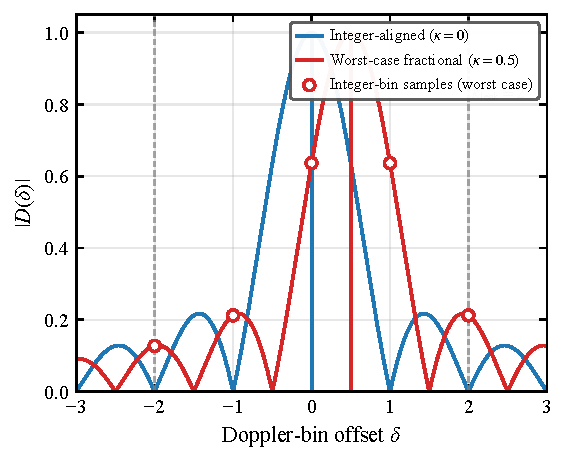
\includegraphics[width=0.55\linewidth]{system_block/fig_dirichlet_kernel.pdf}
\caption{Dirichlet-kernel magnitude $|D(\delta)| = |\sin(\pi\delta) / (\Nsub \sin(\pi\delta / \Nsub))|$ from \eqref{eq:dirichlet} at $\Nsub = 1024$, plotted against the integer-Doppler offset $\delta$. Two cases are overlaid: the integer-aligned residual ($\kappa = k_p^{\text{real}} - k_p = 0$, blue), where the kernel collapses to a sampling indicator and an integer-Doppler dictionary loses no per-path energy; and the worst-case fractional residual ($|\kappa| = 0.5$, red), where the integer-bin samples (red circles) at $\delta \in \{0, +1\}$ each carry $\approx 41\%$ of per-path energy and the samples at $\delta \in \{-1, +2\}$ each carry $\approx 4.4\%$. The dashed vertical lines mark the $\kleak = 2$ truncation boundary used by the simulator; the two-sided sum of squared truncated coefficients beyond $|\delta| > \kleak$ amounts to $\approx 8.3\%$ of per-path energy at $|\kappa| = 0.5$, the figure quoted in the paragraph above. The non-zero side-lobes flanking the kernel peak are the structurally predictable energy that the post-OMP virtual-tap expansion (\S\ref{ssec:joint}) and the learned support-refinement ranker (\S\ref{ssec:c2rel}) are designed to recover.}
\label{fig:dirichlet}
\end{figure}

The geometry summarised in Fig.~\ref{fig:dirichlet} is the physical reason why a single OMP pass on the integer-Doppler dictionary cannot fully resolve the effective channel under fractional Doppler: at the worst-case residual the side-lobe samples adjacent to a main-lobe atom each carry energy comparable to a separate weak path, yet sit at deterministic integer offsets from that already-active atom. This structural predictability motivates the support-refinement head of \S\ref{ssec:c2rel} and is the geometric anchor used by the mechanism discussion in \S\ref{ssec:disc_head}.

\subsection{Superimposed pilot signal model}
\label{ssec:sp}

To preserve spectral efficiency, every chirp-domain sub-carrier simultaneously carries data and pilot energy under a fixed superimposed-pilot (SP) frame
\begin{equation}
\mbx \;=\; \sqrt{\rhop}\; \xp \;+\; \sqrt{1 - \rhop}\; \xd, \qquad \rhop \in (0, 1), \label{eq:sp_frame}
\end{equation}
where $\xp$ is a deterministic Zadoff--Chu sequence of root $r = 7$ and length $\Nsub$ normalised to unit energy~\cite{kaleh2005zadoffchu}, and $\xd$ is a QPSK data vector. The canonical pilot power fraction is $\rhop = 0.5$; higher $\rhop$ strengthens the pilot observation at the cost of data energy, and lower $\rhop$ does the converse~\cite{orozco2011superimposed,tugnait2006superimposed}. Under the model~\eqref{eq:afdm_model}, the pilot projection performed at the receiver yields
\begin{equation}
\xp^H \mby \;=\; \sqrt{\rhop}\; \xp^H \Heff \xp \;+\; \sqrt{1 - \rhop}\; \xp^H \Heff \xd \;+\; \xp^H \mbn, \label{eq:pilot_projection}
\end{equation}
so that the data term $\sqrt{1 - \rhop}\, \xp^H \Heff \xd$ enters as structured interference to the OMP dictionary correlator. Treating $\xd$ as a QPSK data vector independent of $\xp$ with covariance $\E[\xd \xd^H] = (1/\Nsub) \mathbf{I}_{\Nsub}$, the conditional second moment of the interference term given the channel is
\begin{equation}
\E\bigl[\,|\sqrt{1-\rhop}\, \xp^H \Heff \xd|^2\,\big|\,\Heff\bigr] \;=\; (1-\rhop) \cdot \|\Heff^H \xp\|^2 / \Nsub, \label{eq:interferencevar}
\end{equation}
which scales with the channel norm $\|\Heff\|$ and the pilot autocorrelation, and does not shrink with increasing $\snr$. At the canonical operating point ($\rhop = 0.5$, $\Ppath = 8$, $\xp$ a unit-norm Zadoff--Chu sequence) the resulting estimation-limited error floor is observed at $\ber \approx 5 \times 10^{-2}$ for a serial OMP+MP receiver from $\snr \geq 15$~dB; this floor is not derived in closed form because $\|\Heff^H \xp\|^2$ depends on the channel realisation and the pilot--channel cross-correlation structure, and is therefore quantified empirically in Chapter~\ref{sec:results}.

\subsection{Sparse-baseline OMP dictionary}
\label{ssec:dictionary}

The OMP dictionary $\mbPhi \in \C^{\Nsub \times Q}$ is constructed column-wise by evaluating the chirp-domain response of every candidate $(l, k)$-bin in the physical integer search region
\begin{equation}
l \in \{0, 1, \dots, \lmax - 1\}, \qquad k \in \{-\kmax, \dots, \kmax\},
\end{equation}
so that the dictionary size is $Q = (2\kmax + 1) \cdot \lmax$. The dictionary spans physical integer delay--Doppler bins only; the Dirichlet expansion \eqref{eq:dirichlet} is applied post-OMP to each selected atom, so the fractional-Doppler half-width $\kleak$ does not enlarge the dictionary and enters only through the $(2\kleak{+}1)$-fold virtual-tap replication used in the DA-LS refit and MP-BP blocks of \S\ref{ssec:joint}. The caps $\lmax$ and $\kmax$ follow directly from the physical channel parameters,
\begin{align}
\lmax &= \lceil \tau_{\text{spread}} \cdot \fs \rceil, \label{eq:lmax} \\
\kmax &= \left\lceil \frac{v_{\max}\, \fc\, \Nsub}{c\, \fs} \right\rceil, \label{eq:kmax}
\end{align}
and have a consequence that is central to the complexity argument in \S\ref{ssec:complexity}. Holding the sampling rate $\fs$ fixed at the $\fs = 4B$ operating point used throughout this report, $\lmax$ is a constant independent of $\Nsub$, while $\kmax \propto \Nsub / \fs$ grows linearly with $\Nsub$. Therefore
\begin{equation}
Q \;=\; (2\kmax + 1) \cdot \lmax \;=\; \mathcal{O}(\Nsub) \cdot \mathcal{O}(1) \;=\; \mathcal{O}(\Nsub). \label{eq:Qlinear}
\end{equation}
Table~\ref{tab:dictsize} reports the resulting $(\lmax, \kmax, Q)$ triples at $\Nsub \in \{512, 1024, 2048\}$ under the canonical $\fs = 4B$ setting.

\begin{table}[t]
\centering
\caption{OMP dictionary size under the canonical AFDM configuration used throughout this report ($\tau_{\text{spread}} = 10$~ms, $v_{\max} = 3$~m/s, $\fc = 12$~kHz, $\fs = 4B = 16$~kHz). Under the fixed-$\fs$ convention, $\lmax = \lceil \tau_{\text{spread}} \fs \rceil = 160$ is independent of $\Nsub$, while $\kmax = \lceil v_{\max}\fc\Nsub/(c\fs)\rceil$ grows linearly with $\Nsub$. The Chapter~\ref{sec:results} operating point ($\Nsub = 1024$) corresponds to the middle row.}
\label{tab:dictsize}
\begin{tabular}{rrrr}
\toprule
$\Nsub$ & $\lmax$ & $\kmax$ & $Q = (2\kmax+1)\lmax$ \\
\midrule
512  & 160 & 1 & 480   \\
1024 & 160 & 2 & 800   \\
2048 & 160 & 4 & 1\,440 \\
\bottomrule
\end{tabular}
\end{table}

The asymptotic claim $Q = \mathcal{O}(\Nsub)$ is invariant across the two natural UWA conventions: under fixed-$\fs$ as above, and under fixed sub-carrier spacing $\Delta f$ (so that $\fs = \Nsub \Delta f$), in which case $\lmax \propto \Nsub$ and $\kmax = \mathcal{O}(1)$ and the product $Q = (2\kmax{+}1)\lmax = \mathcal{O}(\Nsub)$ still holds. The hidden leading constants differ between the two conventions and are not interchangeable when quoting per-frame multiply-accumulate (MAC) counts.

Each OMP iteration evaluates $\mbPhi^H \mathbf{r}$ at a cost of $\mathcal{O}(\Nsub Q)$ complex multiplications and solves an $s\times s$ least-squares system at $\mathcal{O}(\Nsub s + s^3)$ for the standard direct factorisation, where $s \leq \Ppath$ is the current support size. Running OMP to a target sparsity of $\Ppath = 8$ therefore costs
\begin{equation}
C_{\text{OMP}} \;=\; \mathcal{O}(\Ppath \Nsub Q + \Ppath^4) \;=\; \mathcal{O}(\Ppath \Nsub^2) \label{eq:omp_cost}
\end{equation}
per frame under \eqref{eq:Qlinear}, where the $\Ppath^4$ term is absorbed because $\Ppath \ll \Nsub$ at every operating point used in this report.

\subsection{Joint OMP-once + iterative LS/MP-BP receiver}
\label{ssec:joint}

The receiver performs one OMP support-recovery pass and then iterates only over the data-aided path-gain least-squares (DA-LS) refit and the sparse MP-BP detection block. Algorithm~\ref{alg:joint} summarises the recipe.

\begin{algorithm}[t]
\caption{Classical joint OMP-once + iterative LS/MP-BP receiver.}
\label{alg:joint}
\begin{small}
\textbf{Input}: $\mby$ (chirp-domain received frame), $\mbPhi$ (OMP dictionary), known $\xp$, pilot power $\rhop$. \\
\textbf{Output}: hard-decision data bits $\hat{\xd}$. \\
\textbf{Hyperparameters}: outer iterations $T_\text{out} = 5$, MP inner iterations $T_\text{mp} = 20$, damping $\gamma_h = 0.7$, prune threshold $\tau_h = 10^{-2}\cdot \max |\hat{h}|$.
\begin{enumerate}[leftmargin=*,itemsep=1pt,topsep=2pt]
  \item \textbf{OMP-once}: run orthogonal matching pursuit on $\mbPhi$ with target sparsity $\Ppath$; obtain support $\hat{S}^{(0)}$ and path gains $\hat{\mbh}^{(0)}$. Initialise $\hat{\xd}^{(0)}$ with an LMMSE solution on $\hat{S}^{(0)}$.
  \item \textbf{For} $t = 1, \dots, T_\text{out}$:
  \begin{enumerate}[leftmargin=*,itemsep=1pt,topsep=2pt]
    \item Form the data-cancellation residual
    \begin{equation}
    \mathbf{r}^{(t)} \;=\; \mby \;-\; \sqrt{1-\rhop}\, \Heff(\hat{\mbh}^{(t-1)})\, \hat{\xd}^{(t-1)},
    \label{eq:dals_resid}
    \end{equation}
    where $\hat{\xd}^{(0)}$ is the LMMSE initialisation from step~1; the $\sqrt{\rhop}\,\xp$ pilot contribution is retained in $\mathbf{r}^{(t)}$ because $\xp$ is absorbed into the OMP dictionary $\mbPhi$ (each column carries its pilot-aware atom vector), so the data-interference term is the only component that must be cancelled explicitly.
    \item Damped DA-LS refit on the current support $\hat{S}^{(t-1)}$:
    \begin{equation}
    \hat{\mbh}^{(t)} \;=\; (1-\gamma_h)\,\hat{\mbh}^{(t-1)} \;+\; \gamma_h \cdot \mbPhi_{\hat{S}^{(t-1)}}^{\dagger}\, \mathbf{r}^{(t)}.
    \label{eq:dals}
    \end{equation}
    \item MP-BP on the sparse factor graph $(\Heff(\hat{\mbh}^{(t)}), \mby)$ for $T_\text{mp}$ iterations with damping $0.5$; update posterior means $\hat{\xd}^{(t)}$ and per-symbol variances $\sigma_{d,i}^2$.
    \item Adaptive $\sigma^2$ update; prune atoms with $|\hat{h}_s^{(t)}| < \tau_h$ (always retain the top-$\Ppath$).
  \end{enumerate}
  \item Hard-decide $\hat{\xd} = \mathrm{QPSK\text{-}demap}(\hat{\xd}^{(T_\text{out})})$.
\end{enumerate}
\end{small}
\end{algorithm}

\begin{figure}[t]
\centering
\includegraphics[width=\linewidth]{system_block/figure_a_new.png}
\caption{Classical OMP-once + iterative LS/MP-BP joint receiver (Algorithm~\ref{alg:joint} in block-diagram form). The outer loop (dashed rectangle) runs for $T_\text{out} = 5$ iterations; each iteration forms a data-cancellation residual, refits the path gains on a locked support via damped DA-LS, runs sparse MP-BP detection on the Dirichlet-expanded virtual-tap factor graph, updates the adaptive noise-variance estimate, and prunes the support.}
\label{fig:classical_joint_arch}
\end{figure}

\paragraph{MP-BP messages on the sparse chirp-domain factor graph.}
The data-detection block of Algorithm~\ref{alg:joint} follows the iterative-receiver framework of Wymeersch~\cite{wymeersch2007iterativereceiver} and the factor-graph paradigm surveyed by Kschischang~\emph{et~al.}~\cite{kschischang2001factorgraph}, and is implemented as Gaussian message passing on a bipartite factor graph derived from the pilot-subtracted observation. Subtracting the estimated pilot contribution from~\eqref{eq:afdm_model} yields, for every $j \in \{0, \dots, \Nsub - 1\}$,
\begin{equation}
\tilde{y}_j \;:=\; y_j - \sqrt{\rhop}\, [\Heff(\hat{\mbh}^{(t)})\, \xp]_j \;=\; \sum_{i \in \mathcal{N}(j)} \tilde{H}_{j,i}\, x_{d,i} \;+\; n_j, \label{eq:mpbp_input}
\end{equation}
where $\tilde{H}_{j,i} := \sqrt{1-\rhop}\, [\Heff(\hat{\mbh}^{(t)})]_{j,i}$ absorbs the data-power normalisation and $\mathcal{N}(j) := \{i : \tilde{H}_{j,i} \neq 0\}$ is the index set of variables coupled to factor $j$. The factor graph carries $\Nsub$ variable nodes (one per data symbol $x_{d,i}$) and $\Nsub$ factor nodes (one per row of~\eqref{eq:mpbp_input}). The neighbourhood degree is bounded by $|\mathcal{N}(j)| \leq \Ppath \cdot (2\kleak + 1) = 40$ in the nominal Dirichlet expansion and averages $\preal \approx 28$ per frame after pruning of negligible Dirichlet-weighted entries (App.~\ref{app:recall}); both bounds are constants in $\Nsub$, which is the property that enables $\mathcal{O}(\Nsub)$ per-iteration message passing.

At inner iteration $\ell$, the variable-to-factor message from $x_{d,i}$ to factor $j$ is parameterised as a Gaussian with mean $\mu_{i \to j}^{(\ell)}$ and variance $v_{i \to j}^{(\ell)}$, obtained by aggregating all incoming factor-to-variable messages with the one returning from $j$ excluded:
\begin{equation}
\frac{1}{v_{i \to j}^{(\ell)}} \;=\; \!\sum_{j' \in \mathcal{M}(i) \setminus \{j\}}\! \frac{1}{v_{j' \to i}^{(\ell-1)}}, \qquad \frac{\mu_{i \to j}^{(\ell)}}{v_{i \to j}^{(\ell)}} \;=\; \!\sum_{j' \in \mathcal{M}(i) \setminus \{j\}}\! \frac{\mu_{j' \to i}^{(\ell-1)}}{v_{j' \to i}^{(\ell-1)}}, \label{eq:mpbp_var}
\end{equation}
where $\mathcal{M}(i) := \{j : i \in \mathcal{N}(j)\}$ shares the same constant degree bound. The factor-to-variable message marginalises the row-$j$ Gaussian likelihood over all variables in $\mathcal{N}(j) \setminus \{i\}$,
\begin{align}
\mu_{j \to i}^{(\ell)} &\;=\; \frac{1}{\tilde{H}_{j,i}} \left( \tilde{y}_j - \!\!\sum_{i' \in \mathcal{N}(j) \setminus \{i\}}\!\! \tilde{H}_{j, i'}\, \mu_{i' \to j}^{(\ell)} \right),
\label{eq:mpbp_fact_mean} \\
v_{j \to i}^{(\ell)} &\;=\; \frac{1}{|\tilde{H}_{j,i}|^2} \left( \hat{\sigma}_n^2 + \!\!\sum_{i' \in \mathcal{N}(j) \setminus \{i\}}\!\! |\tilde{H}_{j, i'}|^2\, v_{i' \to j}^{(\ell)} \right), \label{eq:mpbp_fact_var}
\end{align}
where $\hat{\sigma}_n^2$ is the adaptive noise-variance estimate updated at the end of each outer iteration. Both message updates are damped with $\eta = 0.5$ to suppress oscillations on the short cycles characteristic of the Dirichlet-expanded factor graph, $\mu_{i \to j}^{(\ell)} \leftarrow \eta\, \tilde{\mu}_{i \to j}^{(\ell)} + (1-\eta)\, \mu_{i \to j}^{(\ell-1)}$ and analogously for the variances, where $\tilde{\mu}_{i \to j}^{(\ell)}$ denotes the undamped update of~\eqref{eq:mpbp_var}. After $T_\text{mp} = 20$ inner iterations, the posterior on each data symbol is read off by aggregating all incoming factor messages,
\begin{equation}
\frac{1}{\sigma_{d,i}^2} \;=\; \!\sum_{j \in \mathcal{M}(i)}\! \frac{1}{v_{j \to i}^{(T_\text{mp})}}, \qquad \frac{\hat{x}_{d,i}}{\sigma_{d,i}^2} \;=\; \!\sum_{j \in \mathcal{M}(i)}\! \frac{\mu_{j \to i}^{(T_\text{mp})}}{v_{j \to i}^{(T_\text{mp})}}, \label{eq:mpbp_post}
\end{equation}
followed by a Gray-coded QPSK projection $\hat{x}_{d,i} \mapsto \mathrm{QPSK\text{-}demap}(\hat{x}_{d,i})$ that returns the hard-decision data symbol. The Gaussian approximation maintained throughout the inner loop is the standard soft-Gaussian belief-propagation form for finite-alphabet symbols~\cite{wymeersch2007iterativereceiver}, with the QPSK constraint enforced only at the final projection. Because $|\mathcal{N}(j)|$ and $|\mathcal{M}(i)|$ are bounded by constants independent of $\Nsub$, each inner iteration evaluates $\mathcal{O}(\preal \cdot \Nsub)$ scalar updates across all factor and variable nodes, so the data-detection block costs $\mathcal{O}(T_\text{mp} \Nsub)$ per outer iteration. This is the source of the $\mathcal{O}(T_\text{mp} \Nsub)$ term in the per-frame budget of~\eqref{eq:classcomplex}, and it is two orders of magnitude cheaper than a chirp-domain dense MMSE equaliser's $\mathcal{O}(\Nsub^3)$ at $\Nsub = 1024$.

Four design choices in Algorithm~\ref{alg:joint} are central to the receiver's behaviour, and each rejects a simpler or more expensive alternative on empirical or analytical grounds. The OMP-once choice rests on a stability observation: the empirical support Jaccard between successive OMP passes in a hypothetical full re-OMP schedule exceeds $0.94$ from iteration~2 onwards (Fig.~\ref{fig:iterconv}), so the atoms within the support are already stable after a single pass and the only quantity that continues to evolve is the per-path gain amplitude. Chapter~\ref{sec:results}~(\S\ref{ssec:probes}) confirms this independently: OMP-once recovers a mean $\approx 95\%$ recall against the effective Dirichlet-expanded virtual-tap oracle support across all training SNRs (Table~\ref{tab:supportrecall}), so a second OMP pass has nothing new to find. Re-running OMP across outer iterations therefore re-solves a near-identical atom-selection problem $T_\text{out} = 5$ times per frame at a constant-factor overhead of $\sim 5\times$~\eqref{eq:omp_cost} without any change in asymptotic class. Once the support is locked, the path gains are refined by a damped DA-LS update rather than a full LS solve: a full LS over the unrestricted dictionary would amplify noise from unexplored columns, whereas the DA-LS refit \eqref{eq:dals} on the locked support uses exactly the $\Ppath \approx 8$ physical (or $\approx 28$ virtual) taps from step~1 and keeps the gain-update cost at $\mathcal{O}(\Ppath^2 \Nsub)$.

The detection block is sparse MP-BP rather than a dense chirp-domain equaliser. The factor graph induced by $\Heff(\hat{\mbh}^{(t)})$ carries at most $\Ppath \cdot (2\kleak+1) = 40$ non-trivial symbol-to-symbol edges per row in the nominal Dirichlet expansion, with the empirical effective edge count after pruning of negligible Dirichlet weights averaging $\approx 28$ per frame (App.~\ref{app:recall}, $p_{\text{real}}$); the count is constant in $\Nsub$, so each MP-BP iteration costs $\mathcal{O}(\Nsub)$, against the $\mathcal{O}(\Nsub^3)$ per frame of a dense MMSE equaliser --- two full orders of magnitude more expensive at $\Nsub = 1024$. The choice of SP over an embedded-pilot frame is, finally, the source of the data-interference term that motivates iteration in the first place: under EP the OMP step is clean but the spectral efficiency drops by a factor proportional to the pilot fraction, and in a UWA context guard regions also produce artefacts on Dirichlet-expanded virtual taps; SP preserves full data capacity at the cost of the structured interference term \eqref{eq:pilot_projection}, which the iterative recipe is specifically designed to attenuate via successive hard-decision feedback.

\subsection{Learned support-refinement head}
\label{ssec:c2rel}

Even with iteration, the classical joint receiver retains a residual support-selection gap at high SNR, where OMP occasionally misses weak but non-negligible Dirichlet-leakage atoms (typically at $\pm 1$-bin Doppler offsets around the integer-$\kmax$ index) whose estimated gains fall just below $\tau_h$ and are pruned by the gain-magnitude rule. This gap is closed by the \LearnedHead{}: a 1\,041-parameter deep-unfolding module that scores off-support candidates against the currently active support and appends the highest-ranked $\Kadd$ atoms at the initialisation step ($t = 0$), immediately after OMP-once and before the iterative LS/MP-BP loop begins (Fig.~\ref{fig:pipeline_integration}).

\begin{figure}[t]
\centering
\includegraphics[width=\linewidth]{system_block/figure_b_new.png}
\caption{Integration of the learned support-refinement head into the classical OMP-once + iterative LS/MP-BP receiver. The learned block (dark blue) is invoked twice at the initialisation step ($t = 0$), immediately after OMP-once and before the iterative LS/MP-BP loop begins; it ranks the top-$M = 96$ off-support candidates and appends the top-$\Kadd$ atoms to the support. All other blocks are identical to Fig.~\ref{fig:classical_joint_arch}: the head replaces neither OMP-once nor the iterative LS/MP-BP block. The detailed head architecture is given in Fig.~\ref{fig:head_arch}.}
\label{fig:pipeline_integration}
\end{figure}

\begin{figure}[t]
\centering
\includegraphics[width=\linewidth]{system_block/figure_c_new.png}
\caption{Learned support-refinement head (architecture). Two parallel inputs per candidate $i$: a 7-D self-feature $\mathbf{u}_i$ and a set of 6-D pair features $\{\mathbf{v}_{i,s}\}_{s \in \hat{S}}$ indexed over the current active support $\hat{S}$. The shared pair-encoder ($\mathbb{R}^6 \!\to\! \mathbb{R}^{16} \!\to\! \mathbb{R}^{16}$, 384 parameters) is applied element-wise over $(i, s)$ pairs; order-invariant pooling (concat of channel-wise max and mean over $s \in \hat{S}$) produces a 32-D pair descriptor per candidate, which is concatenated with $\mathbf{u}_i$ to form $\boldsymbol{\phi}_i \in \mathbb{R}^{39}$. The shared scorer ($\mathbb{R}^{39} \!\to\! \mathbb{R}^{16} \!\to\! \mathbb{R}^1$, 657 parameters) emits a scalar logit $s_i$; the deterministic top-$\Kadd$ ranker selects the atoms to append. Total trainable parameters: $384 + 657 = 1\,041$. The logits are used only for ranking.}
\label{fig:head_arch}
\end{figure}

\paragraph{Features.}
Let $M$ denote the number of off-support candidate atoms at iteration~$t$; the deployed receiver fixes $M = 96$ by retaining the top-$96$ residual-correlation candidates. For each candidate $i \in \{1, \dots, M\}$ a 7-dimensional self-feature $\mathbf{u}_i \in \R^{7}$ is constructed from
\begin{enumerate}[leftmargin=*,itemsep=0pt,topsep=1pt]
  \item the log matched-filter magnitude $\log |\mbPhi_i^H \mathbf{r}^{(t)}|$;
  \item the margin to the weakest active atom, $\log |\mbPhi_i^H \mathbf{r}^{(t)}| - \min_{s \in \hat{S}} \log |\hat{h}_s|$;
  \item the normalised delay bin index $l_i / \lmax$;
  \item the normalised Doppler bin index $(k_i + \kmax) / (2\kmax)$;
  \item the residual projection norm $\|\mbPhi_i^H \mathbf{r}^{(t)}\| / \|\mathbf{r}^{(t)}\|$;
  \item the candidate rank among the $M$ atoms, normalised to $[0, 1]$;
  \item a binary flag indicating whether $(l_i, k_i)$ lies within $\kleak$ Doppler bins of some active atom (Dirichlet-leakage neighbour).
\end{enumerate}
For each (candidate, active atom) pair $(i, s)$ a 6-dimensional pair feature $\mathbf{v}_{i,s} \in \R^{6}$ is computed:
\begin{equation}
\mathbf{v}_{i,s} =
\bigl[
l_i-l_s,\;
k_i-k_s,\;
\log |\hat{h}_s|,\;
|\mbPhi_i^H \mbPhi_s|,\;
\frac{\|(l_i-l_s,\; k_i-k_s)\|_2}{\lmax + 2\kmax},\;
\frac{|\hat{h}_s|}{\max_{s'} |\hat{h}_{s'}|}
\bigr].
\label{eq:pairfeature}
\end{equation}

\paragraph{Feature design rationale.}
The 7-dimensional self-feature and 6-dimensional pair feature are organised as three complementary information channels that the scorer needs in order to discriminate Dirichlet side-lobe atoms from noise-driven candidates. Self-features 1, 2, and 5 expose the candidate's data-driven correlation strength against three different normalisations: the absolute matched-filter magnitude $\log|\mbPhi_i^H \mathbf{r}^{(t)}|$, the margin against the weakest active atom $\log|\mbPhi_i^H \mathbf{r}^{(t)}| - \min_{s \in \hat{S}} \log|\hat{h}_s|$ that places the candidate on the same logarithmic axis as the active support's tail, and the residual-normalised projection $\|\mbPhi_i^H \mathbf{r}^{(t)}\|/\|\mathbf{r}^{(t)}\|$ that controls for the overall residual energy at iteration $t$. Self-features 3 and 4, the normalised delay and Doppler indices $l_i / \lmax$ and $(k_i + \kmax)/(2\kmax)$, locate the candidate on the physical lattice and let the scorer learn position-dependent priors --- for instance, that bins near $\pm \kmax$ are more likely to host fractional-leakage residuals than bins near zero. Self-feature 6, the candidate's rank among the $M = 96$ retained atoms, provides a tie-breaker that lets the scorer condition on whether a candidate sits near the top of the matched-filter shortlist or at its tail. Self-feature 7, the binary indicator that $(l_i, k_i)$ lies within $\kleak$ Doppler bins of an active atom, is the most directly mechanism-coupled feature: it flags the geometric signature of a Dirichlet side-lobe neighbour and is the feature that most cleanly distinguishes the high-SNR exploitable regime from the low-SNR noise-dominated regime developed in \S\ref{ssec:disc_head}.

The 6-dimensional pair feature $\mathbf{v}_{i,s}$ extends the same reasoning to the relational structure between candidate $i$ and each active atom $s$. The integer offsets $(l_i - l_s, k_i - k_s)$ are the direct encoding of the $(\Delta l, \Delta k) = (0, \pm 1)$ Dirichlet side-lobe signature; combined with the active atom's log-gain $\log|\hat{h}_s|$ and its gain prominence $|\hat{h}_s| / \max_{s'}|\hat{h}_{s'}|$, they let the scorer learn that a candidate at $(0, \pm 1)$ offset from a high-gain active atom is far more likely to be a side-lobe than the same candidate at the same offset from a weak active atom. The pair correlation $|\mbPhi_i^H \mbPhi_s|$ measures dictionary-column similarity directly and supplements the integer-offset signal with a continuous coherence measure, so that pairs of atoms whose chirp-domain responses overlap geometrically can be flagged even when the integer-offset pattern is ambiguous. The normalised Euclidean distance $\|(l_i - l_s,\, k_i - k_s)\|_2 / (\lmax + 2\kmax)$ provides a single scalar that the order-invariant pooling of the architecture (described next) can aggregate across all $|\hat{S}|$ active atoms without losing the geometric information. Taken together, the feature design encodes the rule that a candidate should be promoted when it is a low-Hamming-distance Doppler neighbour of an active atom of non-trivial gain and when its matched-filter response sits above the active-set tail; this is the rule that the oracle-headroom analysis of \S\ref{ssec:probes} validates as covering the bulk of the achievable support-refinement gap, and it is the rule that the scorer is trained to recover.

\paragraph{Architecture.}
The head consists of a shared pair encoder followed by a per-candidate scorer. The pair encoder, denoted $f_{\text{pair}}: \R^{6} \to \R^{16} \to \R^{16}$ with SiLU activation~\cite{elfwing2018silu} after each linear layer, is applied element-wise to every pair feature $\mathbf{v}_{i,s}$, contributing $(6 \cdot 16 + 16) + (16 \cdot 16 + 16) = 384$ parameters. For each candidate $i$, the resulting set of $|\hat{S}|$ per-pair 16-vectors is aggregated into a 32-dimensional pair descriptor by concatenating the element-wise maximum and the element-wise mean across $s$, with no additional trainable parameters. The pooled descriptor is concatenated with the 7-dimensional self-feature $\mathbf{u}_i$ to form a 39-dimensional vector and passed through the scorer $f_{\text{score}}: \R^{39} \to \R^{16} \to \R^{1}$ (SiLU after the first linear; zero-initialised output weights; output bias initialised at $-8$), contributing $(39 \cdot 16 + 16) + (16 \cdot 1 + 1) = 657$ parameters. The total trainable parameter count is $384 + 657 = 1\,041$, of which $\approx 37\%$ sit in the pair encoder and $\approx 63\%$ in the scorer.

\paragraph{Inference.}
The head is deployed as a deterministic fixed-budget top-$\Kadd$ ranker with $\Kadd = 4$: the scorer logits rank the $M = 96$ off-support candidates on every frame, and the top $\Kadd = 4$ logits are appended to the active support without any per-candidate probability thresholding. At outer iteration $t = 0$ the head is invoked twice (i.e.\ two refinement rounds), with support-pruning deferred until the final outer iteration and the two most recently appended atoms protected from gain-prune; hard-decision symbol feedback is used throughout. The learned final-scorer bias ($\approx -8$) is replaced by $+10$ at inference time so that the top-$\Kadd$ selection always fires, which is mathematically a ranking-preserving threshold shift; the deployment is therefore described as ranking-only rather than as a probability-calibrated detector. The training-objective and inference-objective alignment that this introduces is discussed in \S\ref{ssec:training} and Chapter~\ref{sec:discussion}.

\subsection{Training}
\label{ssec:training}

Per-frame feature caches are harvested by running the classical joint receiver to completion on $(\mathrm{channel}, \mathrm{data}, \mathrm{noise})$ realisations drawn from a dedicated training seed block. Each cached frame carries, per candidate, a binary supervision label $y_i \in \{0, 1\}$ that equals $1$ iff the candidate $(l_i, k_i)$ coincides with an active Dirichlet-weighted ground-truth virtual tap of the true channel. The positive-class rate over the $M = 96$ candidates is $\approx 3\%$, which skews the binary cross-entropy (BCE) objective toward the negative class and accounts for the learned final-scorer bias drifting toward $-8$.

The loss is a weighted sum of per-candidate BCE and a pairwise ranking hinge,
\begin{equation}
\mathcal{L}(\theta) \;=\; \mathcal{L}_{\text{BCE}}(\theta) \;+\; \lambda_{\text{rank}} \cdot \max\bigl(0,\; 1 - \min_{y_i=1} s_i(\theta) + \max_{y_j=0} s_j(\theta)\bigr), \qquad \lambda_{\text{rank}} = 0.5, \label{eq:loss}
\end{equation}
where $s_i(\theta)$ is the scorer logit for candidate $i$ and $\theta$ are the head parameters. Training uses AdamW~\cite{loshchilov2019adamw} with learning rate $10^{-3}$, weight decay $10^{-4}$, batch size $512$ cached frames, for 8 epochs with early stopping on the validation BCE (patience = 2). The cache is split 90/10 frame-level into train/val at fixed seed $13\,579$.

The training cache used for the deployed checkpoint is a 27\,k-frame 4-SNR cache at $\snr \in \{10, 15, 20, 25\}$~dB with per-SNR frame weights $\{0.2, 0.3, 0.3, 0.2\}$, harvested at the $\fs = 4B$ operating point. Covering $\snr = 25$~dB explicitly in the cache is necessary to avoid a slight regression in the head's high-SNR behaviour at the same operating point.

\paragraph{Ranking-only deployment.}
Although the BCE term in \eqref{eq:loss} would in principle support a probability-calibrated interpretation of the scorer output, the deployed head is used purely as a top-$\Kadd$ ranker. The bias-replacement scheme at inference is rank-preserving: writing the final logit as $s_i = z_i + b$, replacing $b_{\text{learned}} \approx -8$ by $b_{\text{patch}} = +10$ is a uniform translation of every candidate's logit, which leaves the top-$\Kadd$ ordering invariant. The patch's only operational effect is to shift the gate threshold from $z_i > 8$ (rarely satisfied under $b_{\text{learned}}$) to $z_i > -10$ (almost always satisfied), so every frame proceeds to a forced top-$\Kadd$ selection rather than to a no-op gate output. Probability calibration of the scores is out of scope. A principled alternative that aligns training and inference --- a differentiable top-$\Kadd$ loss or a listwise ranking loss --- is identified as future work in Chapter~\ref{sec:conclusion}. The full analytical decomposition of the bias patch into its rank-preservation and gate-toggling components is deferred to App.~\ref{app:topk_patch}.

\subsection{Complexity analysis}
\label{ssec:complexity}

The arithmetic cost of the proposed receiver is the sum of the classical joint cost and the learned-head overhead. From \S\ref{ssec:joint}, the classical joint costs
\begin{equation}
C_{\text{classical}} \;=\; \underbrace{\mathcal{O}(\Ppath \Nsub Q)}_{\text{OMP-once}} \;+\; T_\text{out} \cdot \bigl[\,\mathcal{O}(\Ppath^2 \Nsub)\ \text{DA-LS}\,+\,\mathcal{O}(T_\text{mp} \Nsub)\ \text{MP-BP}\,\bigr] \;=\; \mathcal{O}(\Ppath \Nsub^2) \label{eq:classcomplex}
\end{equation}
per frame, using $Q = \mathcal{O}(\Nsub)$ from \eqref{eq:Qlinear}. The learned head, per refinement round, performs four operations of order $\Nsub$:
(i) candidate-pool selection by computing the residual--dictionary correlation $\mbPhi^H \mathbf{r}$ over the full $Q$-column dictionary at $\mathcal{O}(\Nsub Q)$ and retrieving the top-$M$ off-support candidates by argpartition at $\mathcal{O}(Q)$ (this step is reused if the OMP-once correlation vector is cached across head invocations, otherwise paid once per round);
(ii) $M$ residual projections $\mbPhi_i^H \mathbf{r}$ at $\mathcal{O}(\Nsub)$ each;
(iii) $M \cdot \Ppath$ pair inner products $\mbPhi_i^H \mbPhi_s$ at $\mathcal{O}(\Nsub)$ each, used in the pair feature \eqref{eq:pairfeature};
(iv) $\mathcal{O}(M \Ppath)$ pair-encoder evaluations and $\mathcal{O}(M)$ scorer evaluations of constant per-pair cost.
Summed over the two refinement rounds,
\begin{equation}
C_{\text{head}} \;=\; \mathcal{O}\bigl(\Nsub Q + M \Ppath \Nsub\bigr) \;=\; \mathcal{O}(\Nsub^2) \label{eq:headcomplex}
\end{equation}
under fixed $(M, \Kadd, \Ppath)$ and $\eqref{eq:Qlinear}$, the same asymptotic class as a single OMP-once matched-filter sweep.

The proposed receiver therefore lies in the same $\mathcal{O}(\Ppath \Nsub^2)$ arithmetic class as the sparse classical baseline, and is two orders of magnitude cheaper than a dense LMMSE channel estimator ($\mathcal{O}(\Nsub^3)$) and a $5\times$ constant factor cheaper than a re-OMP-per-iteration schedule. Table~\ref{tab:complexity} in Chapter~\ref{sec:results} tabulates per-frame MAC counts at $\Nsub = 1024$ for these recipes; the proposed learned receiver adds $\approx 1.5$~M MAC on top of the $18.6$~M-MAC classical core, for a relative overhead of $\approx 8\%$. The MAC count is a first-order arithmetic measure; runtime, memory-hierarchy, and energy effects on a realistic embedded target are out of scope here and are discussed in \S\ref{ssec:weaknesses}.

\subsection{Evaluation protocol}
\label{ssec:eval}

All receivers are evaluated under a strict paired-frame protocol. For every $\snr$ point, each of the four receivers (\Serial{}, \ClassicalJoint{}, \LearnedHead{}, \Oracle{}) consumes the same $(\mathrm{channel}, \mathrm{data}, \mathrm{noise})$ realisation drawn from an RNG chained off a master seed (default $20\,260\,425$), so that BER differences across receivers are interpretable frame-by-frame and invariant to channel-draw variance. The default bit budget is $400$~frames~$\times\,2 \cdot 1024 = 8.19 \times 10^{5}$~bits per $\snr$ point.

Reported BERs are observed frequencies $\hat{p} = \text{bit errors}/\text{bits}$. For the headline numbers at $\fs = 4B$, two-sided Clopper--Pearson 95\% confidence intervals are quoted from the exact binomial distribution. Significance between the classical joint and the learned receiver is tested with the continuity-corrected paired McNemar $\chi^2$ on bit-level discordant counts $(n_{10}, n_{01})$; the reported $p$-values are the two-sided asymptotic values, with the within-frame independence assumption, the one-sided exact-binomial complement, and the degenerate-discordants edge case discussed in Appendix~\ref{app:mcnemar}. Where the Monte-Carlo sampling uses an adaptive early-stop rule, the sampler terminates an $\snr$ point only after the classical arm has accumulated a target bit-error budget and a minimum frame count, so the recorded bit budget per point is never smaller than the budget required to make the paired test well-defined.

Train, validation, and test separation is enforced at the seed level. The $\fs = 4B$ feature cache is produced from training seed blocks $20\,260\,420$ and $20\,260\,421$, while all evaluation frames are drawn from a pairwise disjoint set of evaluation seeds: the 3-seed pooled headline in Table~\ref{tab:ber4b} uses evaluation seed blocks $20\,260\,423$, $20\,260\,424$, $20\,260\,425$, and the single-seed illustrative row uses the isolated master seed $20\,260\,425$. Training and evaluation seed blocks are pairwise disjoint by construction; no evaluated $(\mathrm{channel}, \mathrm{data}, \mathrm{noise})$ triple coincides with any training cache frame.

\subsection{Baseline selection and fairness}
\label{ssec:fairness}

Four receivers are compared head-to-head in Chapter~\ref{sec:results}. The \Serial{} arm is the closest single-pass realisation of the classical sparse-recovery literature~\cite{tropp2007signal,berger2010uwasparse} and makes the SP estimation-limited floor explicit. The \ClassicalJoint{} arm is the strongest classical baseline for AFDM-SP that this report constructs; it shares every component with \LearnedHead{} except the head itself, which is precisely the asymmetry needed to attribute observed gains to the learned module. The \Oracle{} arm uses the true $\Heff$ with pilot cancellation and a dense MMSE equaliser as a reference rather than as an information-theoretic lower bound (\S\ref{ssec:weaknesses}).

All four receivers use identical master seeds, identical pilot sequences, identical frame budgets, and identical hyperparameters where applicable: in particular, the classical joint arm is the ablated learned receiver with its head disabled (zero appended atoms and head-logits set to $-\infty$). The only training-time asymmetry is that \LearnedHead{} has seen cached frames at $\snr \in \{10, 15, 20, 25\}$~dB; evaluation points at $\snr \in \{0, 5\}$~dB therefore lie outside the training distribution and are read as out-of-distribution checks rather than in-distribution comparisons. This asymmetry is declared at every table and figure where low-SNR numbers appear.
